\documentclass[11pt]{article}
\usepackage[margin=0.82in]{geometry}
\usepackage{amsmath,amssymb,amsthm,mathtools}
\usepackage{graphicx}
\graphicspath{{figures/}}
\usepackage{booktabs}
\usepackage{microtype}
\usepackage{xcolor}
\usepackage{enumitem}
\usepackage{caption}
\usepackage{hyperref}
\usepackage{array}
\usepackage{lmodern}

\definecolor{navy}{RGB}{30,62,94}
\definecolor{softblue}{RGB}{235,243,252}
\definecolor{softorange}{RGB}{253,246,235}
\definecolor{softgreen}{RGB}{239,248,239}
\hypersetup{colorlinks=true,linkcolor=navy,citecolor=navy,urlcolor=navy}

\newcommand{\E}{\mathbb{E}}
\newcommand{\R}{\mathbb{R}}
\newcommand{\Var}{\operatorname{Var}}
\newcommand{\Id}{\mathrm{I}}
\newcommand{\etal}{\eta_{\mathrm L}}
\newcommand{\etams}{\eta_{2}}
\newcommand{\etah}{\eta_{\mathrm H}}
\newcommand{\etab}{\eta_{\mathrm B}}
\newcommand{\norm}[1]{\left\lVert #1\right\rVert}
\newtheorem{proposition}{Proposition}
\newtheorem{conjecture}{Conjecture}
\newtheorem{definition}{Definition}
\newtheorem{remark}{Remark}

\title{\vspace{-1.2em}\textbf{Shape of SGD Iterates Beyond Stochastic Linear Stability}\\
\large Revised manuscript backbone}
\author{Anonymous authors}
\date{}

\begin{document}
\maketitle
\vspace{-1.5em}

\begin{abstract}
We study the local distribution of stochastic-gradient iterates near a minimizer when the local curvature itself is random.  The linearized dynamics form a random multiplicative cocycle, and therefore stochastic stability is not described by a single edge.  In the scalar model, the $q$-moment edge is determined by $\E|1-\eta h|^q=1$, mean-square stability corresponds to $q=2$, and the pathwise stability edge is the Lyapunov condition $\E\log|1-\eta h|=0$.  These thresholds can be widely separated: the second moment may be unstable while typical trajectories still contract.  Higher-order terms then confine the dynamics after local instability and permit non-Gaussian, heavy-tailed, and eventually two-lobe iterate distributions.  We separate three phenomena: moment instability, loss of typical local stability, and the distributional transition to bimodality.  Experiments with Gaussian, uniform, and scaled chi-square curvature show a common progression from mean-square instability to the Lyapunov edge and then to a delayed central-depletion transition.  We subsequently specialize to deterministic curvature with additive Gaussian noise, where all positive-moment and Lyapunov edges coincide and the existing perturbative theory of noisy flip bifurcations applies.
\end{abstract}

\noindent\colorbox{softorange}{\parbox{0.965\linewidth}{\textbf{Status of this document.} This is a proposed backbone for the revised paper.  Results stated as propositions are standard or directly derivable from the scalar random-product model.  The identification of the exact bimodality threshold with a harmonic quantity is intentionally stated as an empirical observation or a theorem target, because the unregularized negative moment diverges for continuous curvature laws that place density at the cancellation point.}}

\section{Introduction}

Let $L:\R^d\to\R$ be a smooth population loss and let $x^\star$ be a local minimizer.  We consider stochastic-gradient dynamics
\begin{equation}
    X_{t+1}=X_t-\eta\,g(X_t;\xi_t),
    \qquad \E_{\xi}[g(x;\xi)]=\nabla L(x),
    \label{eq:sgd}
\end{equation}
where $\eta>0$ is the step size and $\xi_t$ denotes the sampled mini-batch or stochastic-gradient randomness.  The randomness need not be additive and need not be Gaussian.  Expanding a stochastic gradient around $x^\star$ gives
\begin{equation}
 g(x^\star+\Delta;\xi)
 =g(x^\star;\xi)+H_{\xi}\Delta+N_{\xi}(\Delta),
 \qquad N_{\xi}(\Delta)=O(\norm{\Delta}^2),
 \label{eq:localgrad}
\end{equation}
with stochastic curvature $H_{\xi}=\nabla_xg(x^\star;\xi)$.  Hence the local recursion is
\begin{equation}
 \Delta_{t+1}
 =A_t\Delta_t+\zeta_t+R_t(\Delta_t),
 \qquad
 A_t=\Id-\eta H_{\xi_t},
 \quad
 \zeta_t=-\eta g(x^\star;\xi_t),
 \label{eq:localnormal}
\end{equation}
where $R_t(\Delta)=-\eta N_{\xi_t}(\Delta)$.  Equation~\eqref{eq:localnormal} separates three mechanisms:
\begin{enumerate}[leftmargin=1.6em,itemsep=0.15em]
    \item the random linear cocycle $A_t$, which determines local stochastic stability;
    \item the additive residual $\zeta_t$, which may vanish in interpolating problems and is Gaussian only in the additive-noise specialization;
    \item the nonlinear remainder $R_t$, which can arrest the growth caused by linear instability and create off-center metastable states.
\end{enumerate}

This decomposition changes the interpretation of the edge of stability.  For deterministic gradient descent, local stability is controlled by the eigenvalues of one fixed Jacobian.  For SGD, the Jacobian changes with the sampled batch, and the relevant object is the product
\begin{equation}
 A_{t-1}A_{t-2}\cdots A_0.
\end{equation}
Different functionals of this random product produce different critical step sizes.  Mean-square stability controls the second moment, whereas the top Lyapunov exponent controls the growth of a typical infinitesimal perturbation.  Rare curvature samples can destabilize the second moment long before they destabilize a typical trajectory.  Thus moment blow-up, pathwise instability, and bimodality are distinct transitions.

Our scalar canonical model is
\begin{equation}
 X_{t+1}=(1-\eta h_t)X_t+\Phi_\eta(X_t)+\zeta_t,
 \label{eq:scalarcanonical}
\end{equation}
where $h_t$ is a sampled curvature and $\Phi_\eta(x)=O(x^3)$ is a confining nonlinear term.  A polynomial example is obtained from the stochastic local loss
\begin{equation}
 \ell_h(x)=\frac{h}{2}x^2-\frac{\alpha}{4}x^4+\frac{\beta}{6}x^6,
 \qquad \alpha,\beta>0,
\end{equation}
which yields
\begin{equation}
 X_{t+1}=(1-\eta h_t)X_t+\eta\alpha X_t^3-\eta\beta X_t^5+\zeta_t.
 \label{eq:polynomialsgd}
\end{equation}


For numerical normal-form experiments, the coefficients of the cubic and quintic terms may equivalently be treated as fixed map coefficients after absorbing their step-size scaling.

The revised paper is organized around the following claim:
\begin{quote}
\emph{The Lyapunov edge determines the loss of typical local stability, but the shape transition to a two-lobe distribution requires additional nonlinear confinement and central-depletion conditions.}
\end{quote}
The additive-Gaussian analysis in the existing manuscript becomes a structured special case rather than the starting point of the theory.

\paragraph{Contributions.}
The proposed paper makes four conceptual contributions.
\begin{enumerate}[leftmargin=1.6em,itemsep=0.25em]
    \item It formulates local SGD as a random-curvature cocycle with optional additive forcing and nonlinear stabilization.
    \item It separates signed-mean stability, positive $q$-moment stability, Lyapunov stability, and a negative-moment anti-reinjection criterion.
    \item It demonstrates a regime in which mean-square stability has already failed but the origin remains Lyapunov stable, followed by a delayed distributional transition to bimodality.
    \item It recovers the current additive-Gaussian flip-bifurcation theory as the deterministic-curvature case in which the positive-moment and Lyapunov thresholds collapse to the same edge.
\end{enumerate}

\section{Stochastic linear stability}

We first remove the nonlinear and additive terms and study
\begin{equation}
    X_{t+1}=A_tX_t,
    \qquad A_t=1-\eta h_t,
    \label{eq:scalarlinear}
\end{equation}
with i.i.d. curvature samples $h_t$.  The scalar setting exposes the complete stability hierarchy and provides the normal-direction theory used later in high dimensions.

\subsection{Positive $q$-moment stability}

For every $q>0$,
\begin{equation}
    \E|X_t|^q=|X_0|^q\left(\E|A|^q\right)^t.
\end{equation}
This motivates the following definition.

\begin{definition}[$q$-moment stability]
For $q>0$, define
\begin{equation}
    m_q(\eta):=\E|1-\eta h|^q.
\end{equation}
The origin is $q$-moment stable when $m_q(\eta)<1$, and the corresponding edge $\eta_q$ solves $m_q(\eta_q)=1$.
\end{definition}

The case $q=2$ is mean-square stability, while $q=1$ is absolute first-moment stability.  This must be distinguished from signed-mean stability:
\begin{equation}
    \E X_t=\left(\E A\right)^tX_0,
    \qquad |\E A|<1.
    \label{eq:signedmean}
\end{equation}
Signed-mean stability can hold because positive and negative multipliers cancel, even while absolute moments and typical trajectories are unstable.

\begin{proposition}[Moment hierarchy]
If $q_2>q_1>0$ and $m_{q_2}(\eta)<1$, then $m_{q_1}(\eta)<1$.  In particular,
\begin{equation}
    \text{mean-square stable}
    \Longrightarrow
    \text{absolute-mean stable}
    \Longrightarrow
    \text{Lyapunov stable}.
    \label{eq:hierarchy}
\end{equation}
\end{proposition}

\noindent The first implication follows from monotonicity of $L^q$ norms.  The second follows from Jensen's inequality:
\begin{equation}
    \E\log|A|\leq \log\E|A|<0.
\end{equation}
The converses fail, and the failure can be arbitrarily large under rare curvature events.

\subsection{The Lyapunov edge as the typical stability limit}

The almost-sure exponential growth rate is
\begin{equation}
    \lambda(\eta)
    :=\lim_{t\to\infty}\frac{1}{t}\log\left|\frac{X_t}{X_0}\right|
    =\E\log|1-\eta h|,
    \label{eq:lyapscalar}
\end{equation}
under the standard integrability condition $\E|\log|1-\eta h||<\infty$.  Thus
\begin{equation}
    \lambda(\eta)<0
    \quad\Longleftrightarrow\quad
    \text{typical local contraction},
\end{equation}
while $\lambda(\eta)>0$ means that the origin is locally repelling for a typical trajectory.  The Lyapunov edge $\etal$ is defined by
\begin{equation}
    \E\log|1-\etal h|=0.
    \label{eq:lyapedge}
\end{equation}
It is also the $q\to0$ limit of the positive moment family:
\begin{equation}
    \lim_{q\to0}\frac{1}{q}\log \E|A|^q=\E\log|A|.
\end{equation}

In multiple dimensions, the scalar expectation is replaced by the top Lyapunov exponent
\begin{equation}
 \lambda_{\mathrm{top}}(\eta)
 =\lim_{t\to\infty}\frac1t
 \log\norm{(\Id-\eta H_{t-1})\cdots(\Id-\eta H_0)},
 \label{eq:toplyap}
\end{equation}
which is the natural stochastic analogue of the largest Jacobian multiplier.

\subsection{The harmonic quantity and central reinjection}

The negative moment
\begin{equation}
    H(\eta):=\E|1-\eta h|^{-1}
    \label{eq:harmonic}
\end{equation}
should not be called an ordinary stability criterion.  It weights near-cancellation events $|1-\eta h|\approx0$ and therefore measures how strongly the dynamics can reinject mass into a neighborhood of the origin.  In transfer-operator arguments, a condition such as $H(\eta)<1$, together with confinement and regularity, can be used as a sufficient central-depletion condition.

For an absolutely continuous curvature density with $f_h(1/\eta)>0$, however,
\begin{equation}
    \E|1-\eta h|^{-1}=\infty.
\end{equation}
Consequently, Gaussian and chi-square curvature do not possess a finite population harmonic edge in the relevant range.  The numerical plots therefore use either a finite-sample proxy
\begin{equation}
    H_M(\eta)=\frac1M\sum_{i=1}^M|1-\eta h_i|^{-1}
\end{equation}
or a regularized quantity $H_\varepsilon(\eta)=\E[(|1-\eta h|\vee\varepsilon)^{-1}]$.  We denote the associated empirical or regularized crossing by $\widehat\eta_{\mathrm H}$.  Establishing a population-level replacement for continuous laws is a central theoretical objective of the revised paper.

\section{Gaussian random curvature: exact mean-square edge and Lyapunov expansion}

Let
\begin{equation}
    h\sim\mathcal N(\mu,s^2).
\end{equation}
The mean-square edge follows exactly from
\begin{align}
 \E(1-\eta h)^2
 &=1-2\eta\mu+\eta^2(\mu^2+s^2).
\end{align}
Setting this equal to one gives
\begin{equation}
    \boxed{\etams=\frac{2\mu}{\mu^2+s^2}}.
    \label{eq:msexact}
\end{equation}
For small curvature variance,
\begin{equation}
    \etams
    =\frac{2}{\mu}-\frac{2s^2}{\mu^3}+O(s^4).
    \label{eq:msexpand}
\end{equation}

For the Lyapunov exponent, expand $g(h)=\log|1-\eta h|$ around $\mu$:
\begin{equation}
 \E g(h)
 =g(\mu)+\frac{s^2}{2}g''(\mu)+O(s^4)
 =\log|1-\eta\mu|
 -\frac{\eta^2s^2}{2(1-\eta\mu)^2}+O(s^4).
 \label{eq:lyapexpand}
\end{equation}
Writing $\etal=2/\mu+\delta$ and solving $\lambda(\etal)=0$ yields
\begin{equation}
    \boxed{\etal=\frac{2}{\mu}+\frac{2s^2}{\mu^3}+O(s^4)}.
    \label{eq:lyapedgeapprox}
\end{equation}
Therefore
\begin{equation}
    \boxed{
    \etams<\frac{2}{\mu}<\etal,
    \qquad
    \etal-\etams=\frac{4s^2}{\mu^3}+O(s^4).}
    \label{eq:gap}
\end{equation}
This is the mathematically clean regime in which the second moment is unstable but a typical trajectory remains locally contracting.

For the experiments with $\mu=1$ and $s^2=0.01$,
\begin{equation}
    \etams=1.980198\ldots,
    \qquad
    \etal\approx2.02,
\end{equation}
with the numerical Gaussian value $\etal\approx2.02116$.

\section{From instability to distributional shape}

We now restore the nonlinear term in~\eqref{eq:scalarcanonical}.  The three relevant transitions are:
\begin{enumerate}[leftmargin=1.6em,itemsep=0.25em]
    \item \textbf{Moment transition:} $\eta=\eta_2$, where the second moment of the linearized recursion loses stability.
    \item \textbf{Typical-stability transition:} $\eta=\etal$, where the top Lyapunov exponent changes sign.
    \item \textbf{Shape transition:} $\eta=\etab$, where the invariant or quasi-stationary density changes from centrally peaked to two-lobed.
\end{enumerate}
For a symmetric density $p_\eta$, a convenient operational definition is
\begin{equation}
    \etab:=\inf\left\{\eta:\ p_\eta(0)<\sup_{x\neq0}p_\eta(x)\right\}.
    \label{eq:bimodaledge}
\end{equation}
When $p_\eta$ is twice differentiable and the transition is local, this corresponds to $p_\eta''(0)$ changing sign.

The Lyapunov condition is the correct necessary local condition for \emph{instability-generated} bimodality: if $\lambda(\eta)<0$, typical sufficiently small perturbations return toward the minimizer.  It is not sufficient.  Beyond $\etal$, nonlinear confinement must create stable off-center dynamics, and curvature randomness must not broaden or reinject enough mass to preserve a dominant central peak.

A useful sufficient-condition program is:
\begin{align}
 &\text{origin instability:} && \E\log|F_h'(0)|>0,\\
 &\text{lobe stability:} && \E\log|(F_{h_2}\circ F_{h_1})'(X^\star)|<0,\\
 &\text{separation:} && F_h(I_+)\subset I_-,\quad F_h(I_-)\subset I_+,
 \quad 0\notin I_+\cup I_-.
 \label{eq:sufficientprogram}
\end{align}
Here $I_-=-I_+$ are separated intervals and $X^\star$ denotes the off-center random attractor.  The interval condition is stronger than necessary but directly implies an alternating two-lobe physical distribution.  A harmonic or regularized anti-reinjection bound may provide a weaker density-based route.

\begin{conjecture}[Delayed shape transition]
For bounded continuous curvature with sufficiently small variance and a smooth confining odd nonlinearity, there is a nonempty interval
\begin{equation}
    \etal<\eta<\etab
\end{equation}
in which the origin is locally Lyapunov unstable but the stationary or quasi-stationary law remains centrally peaked.  The transition at $\etab$ occurs when off-center separation dominates within-lobe broadening and central reinjection.
\end{conjecture}

\begin{figure}[t]
    \centering
    % Upload the figure to the Overleaf project as
    % figures/continuous_curvature_histograms_raw_scientific_with_variable_regimes.png
    % or change the filename below.

    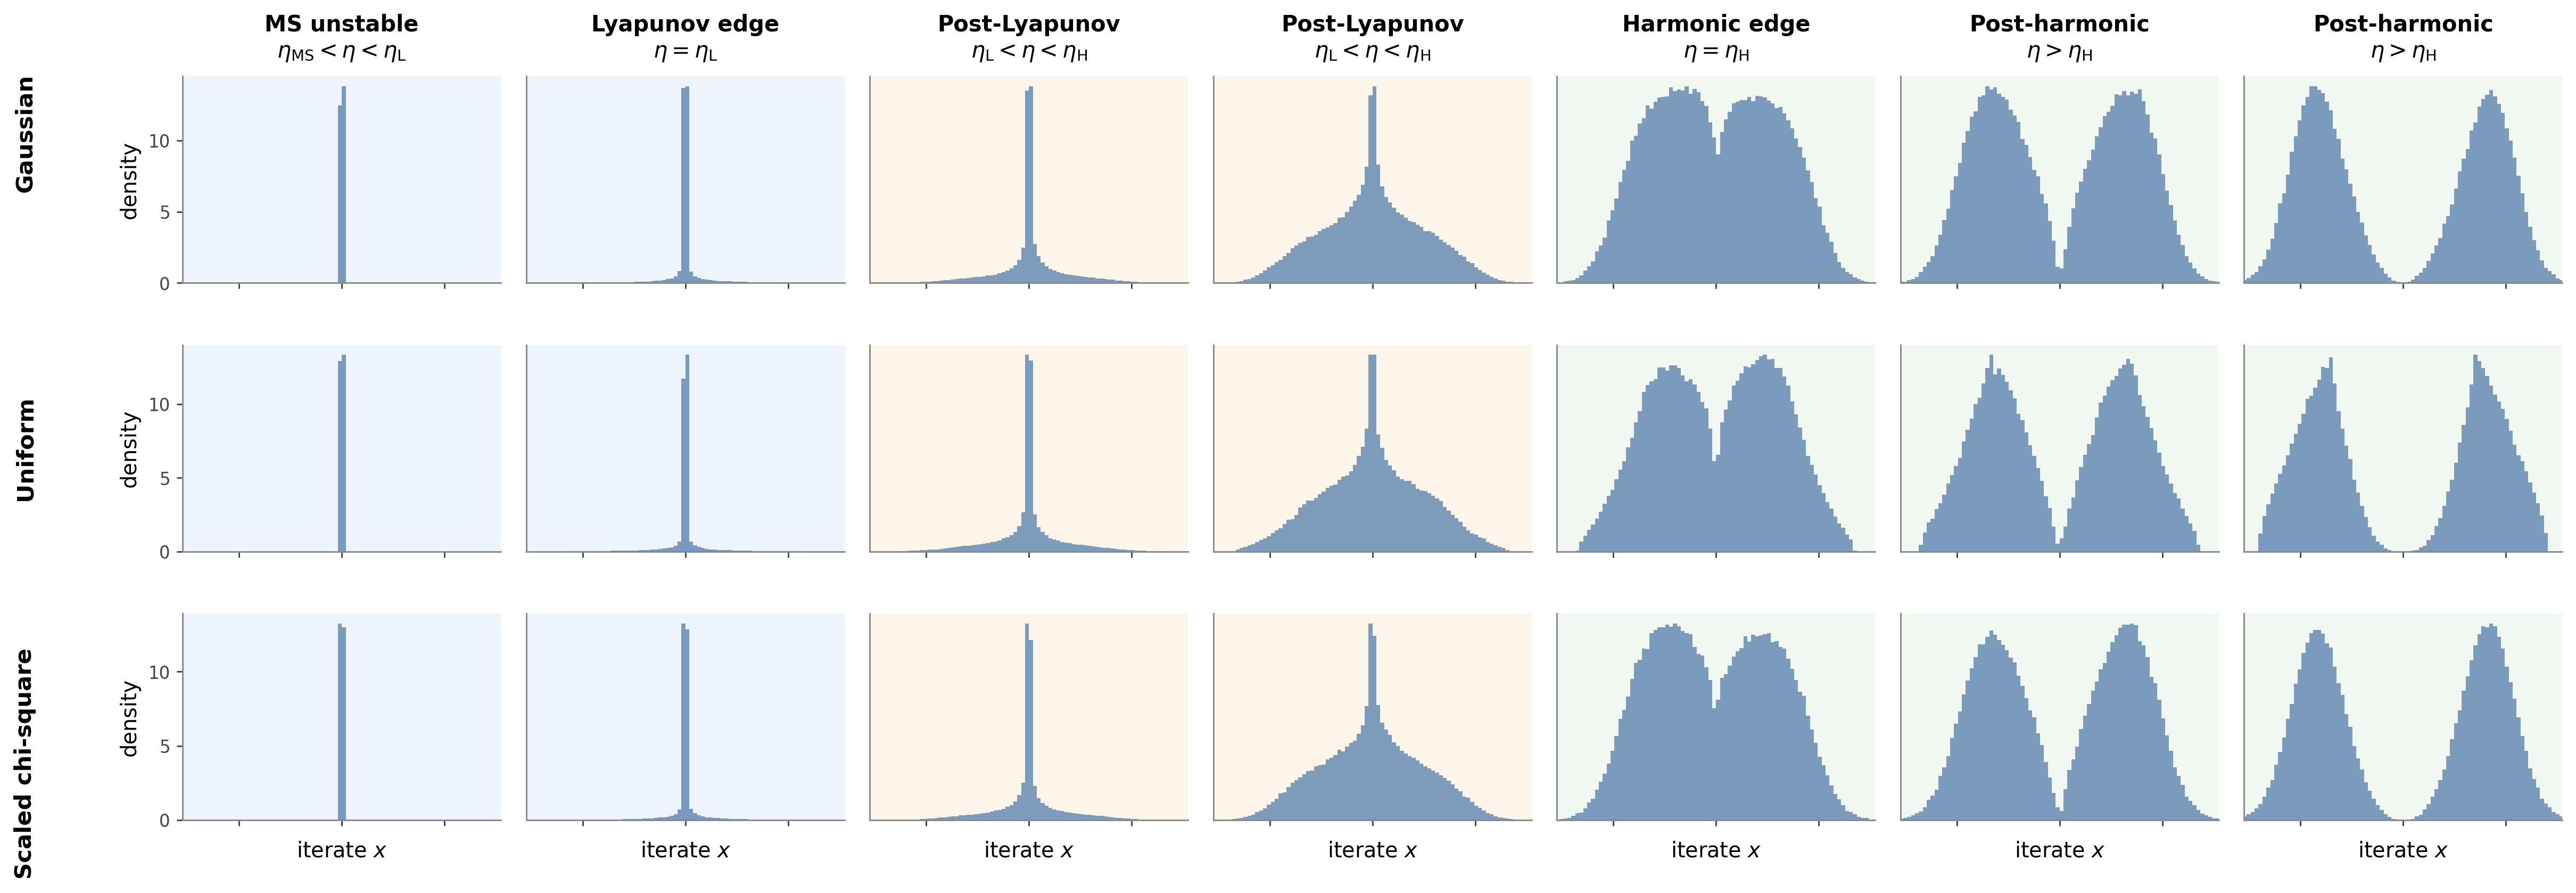
\includegraphics[width=1.0\linewidth]{img/continuous_curvature_histograms_raw_scientific_with_variable_regimes.png}
    \caption{Representative iterate histograms for three continuous random-curvature laws with matched mean and variance.  The first column lies beyond the mean-square edge while remaining Lyapunov stable.  The origin loses typical local stability at $\eta_{\mathrm L}$, but clear two-lobe structure emerges only later.  In this working figure, $\eta_{\mathrm H}$ denotes a finite-sample or regularized harmonic proxy $\widehat\eta_{\mathrm H}$; the population negative moment is divergent whenever the curvature density is nonzero at $h=1/\eta$.  The figure therefore supports a delayed central-depletion transition, not yet an exact population harmonic theorem.}
    \label{fig:histograms}
\end{figure}

\section{Additive Gaussian noise as a special case}

The current manuscript specializes early to additive Gaussian perturbations around a deterministic flip orbit.  In the revised structure, that analysis follows the random-curvature theory as a special case.  Let
\begin{equation}
    X_{t+1}=aX_t+\sigma\xi_t,
    \qquad a=1-\eta h,
    \qquad \xi_t\sim\mathcal N(0,1),
    \label{eq:ar1}
\end{equation}
with deterministic curvature $h$.  The randomness is purely additive, so the Jacobian multiplier is deterministic.  Consequently, for every $q>0$,
\begin{equation}
    |a|^q<1
    \quad\Longleftrightarrow\quad
    |a|<1
    \quad\Longleftrightarrow\quad
    \log|a|<0.
\end{equation}
Thus all positive $q$-moment edges and the Lyapunov edge coincide at
\begin{equation}
    |1-\eta h|=1,
    \qquad \eta=\frac{2}{h}
\end{equation}
for positive step size.  The harmonic equation $|a|^{-1}=1$ has the same boundary location, although its inequality points to the expanding side and should be interpreted as anti-reinjection rather than conventional stability.  The coincidence of the edges is caused by the deterministic Jacobian, not by Gaussianity itself.

Once this common edge is crossed, the deterministic higher-order terms generate a flip orbit under the normal-form condition already proved in the current manuscript.  Additive Gaussian forcing then broadens the two orbit points into two stochastic lobes.  The existing two-step expansion, stopping-time confinement, truncation control, and formulas for the lobe mean and variance can be retained with only a new transition paragraph and updated notation.

\section{Proposed organization of the full paper}

\begin{enumerate}[leftmargin=1.7em,itemsep=0.35em]
    \item \textbf{Introduction and empirical motivation.} Present neural-network iterate histograms and motivate distributional shape beyond a single EoSS threshold.
    \item \textbf{Local stochastic normal form.} Derive~\eqref{eq:localnormal} from generic SGD and distinguish random curvature, additive forcing, and nonlinear stabilization.
    \item \textbf{Stochastic linear stability hierarchy.} Define signed mean, positive $q$ moments, the Lyapunov exponent, and the harmonic/anti-reinjection quantity.  Prove the implication hierarchy and give scalar and multidimensional formulations.
    \item \textbf{Continuous random curvature.} Derive exact and asymptotic thresholds, including~\eqref{eq:msexact}--\eqref{eq:gap}; present histogram and stochastic-bifurcation experiments for Gaussian, uniform, and chi-square laws.
    \item \textbf{Bimodality beyond the Lyapunov edge.} State the necessary Lyapunov condition, formulate invariant-interval or two-step contraction sufficient conditions, and distinguish exact harmonic results from regularized empirical proxies.
    \item \textbf{Additive Gaussian specialization.} Retain the present deterministic flip theorem and the perturbative analysis of the two stochastic lobes, including moment and exit-time control.
    \item \textbf{Multidimensional predictor dynamics.} Retain the current sharp/tangent-coordinate predictor system, but interpret its normal-direction edge through the stochastic Lyapunov framework.
    \item \textbf{Neural-network experiments.} Compare batch sharpness, active-subspace Lyapunov exponents, parity-conditioned iterate distributions, and lobe separation across optimizers and architectures.
\end{enumerate}

\section{Claims that should and should not be made yet}

\begin{center}
\begin{tabular}{>{\raggedright\arraybackslash}p{0.29\linewidth} >{\raggedright\arraybackslash}p{0.31\linewidth} >{\raggedright\arraybackslash}p{0.31\linewidth}}
\toprule
\textbf{Ready to state rigorously} & \textbf{Supported empirically} & \textbf{Theorem target / open point}\\
\midrule
$q$-moment hierarchy and Lyapunov limit & Delayed bimodality after $\etal$ for three continuous laws & Necessary and sufficient conditions for bimodality under general continuous curvature\\[0.35em]
Exact Gaussian mean-square edge and small-variance Lyapunov expansion & Similar shape progression across matched Gaussian, uniform, and chi-square laws & Population-level replacement for the divergent harmonic moment\\[0.35em]
Coincidence of positive-$q$ and Lyapunov edges for deterministic curvature with additive noise & Approximate alignment of central depletion with a finite-sample harmonic proxy & Rigorous invariant density and central-depletion theorem beyond $\etal$\\[0.35em]
Existing additive-Gaussian flip and lobe perturbation theory & Neural-network two-lobe projections & Full-space relation between EoSS, top Lyapunov exponent, and observed lobes\\
\bottomrule
\end{tabular}
\end{center}

\section{Proposed revised paper message}
\enlargethispage{4\baselineskip}

The paper should not claim that mean-square instability is the onset of bimodality, nor that the Lyapunov edge alone is sufficient.  The clean statement is:
\begin{quote}
\emph{Random curvature creates a hierarchy of stochastic stability edges.  Mean-square instability marks a moment transition, the top Lyapunov exponent marks the loss of typical local stability, and nonlinear confinement together with central depletion determines the later transition to a two-lobe iterate distribution.  Purely additive noise is a special case in which the positive-moment and Lyapunov edges coincide.}
\end{quote}
This framing preserves the strongest existing additive-Gaussian results while giving them a broader and more accurate role in a theory of SGD dynamics beyond EoSS.

\end{document}
